\documentclass{article}

\author{Dinh Van Quang}
\date{\today}

\usepackage{amsmath}
\usepackage[english]{babel}
\usepackage[utf8]{inputenc}
\usepackage[document]{ragged2e}
\usepackage{graphicx, color, layout}
\usepackage{listings}

\definecolor{codegreen}{rgb}{0,0.6,0}
\definecolor{codegray}{rgb}{0.5,0.5,0.5}
\definecolor{codepurple}{rgb}{0.58,0,0.82}
\definecolor{backcolour}{rgb}{0.95,0.95,0.92}
\lstdefinestyle{mystyle}{
	backgroundcolor=\color{backcolour},   
	commentstyle=\color{codegreen},
	keywordstyle=\color{magenta},
	numberstyle=\tiny\color{codegray},
	stringstyle=\color{codepurple},
	basicstyle=\footnotesize,
	breakatwhitespace=false,         
	breaklines=true,                 
	captionpos=b,                    
	keepspaces=true,                 
	numbers=left,                    
	numbersep=5pt,                  
	showspaces=false,                
	showstringspaces=false,
	showtabs=false,                  
	tabsize=2
}

\lstset{style=mystyle}

\begin{document}
	\title{description}
	\justify
	
	\section*{Description}
	
	\subsection*{Objectif}
	
	L'intérêt du cas test est de vérifier le calcul TRUST pour la conduction de chaleur anisotrope dans une géométrie assimilé de la couche de diffusion de gaz de PEMFC.
	
	\subsection*{Physique}
	La conduction de la chaleur dans GDL (pemfc) est anisotrope. Le coefficient de conductivité dans le plan (parallèle) de GDL est beaucoup plus élevé que celui perpendiculaire au plan (dans l'ordre de grandeur d'une centaine). De plus, la conduction est réduit lors de l'écrasement du GDL: zone non écrasé est plus conductrice que la zone écrasée. La conductivité dans la zone transitoire est interpolé linéairement.
	
	\paragraph{Géométrie}
	La géométrie utilisée est modélisé d'une partie de GDL écrasé par la plaque bipolaire (en métal) comme montrant la Figure \ref{fig:geom}. 
	
	\begin{figure}[ht]
		\centering
		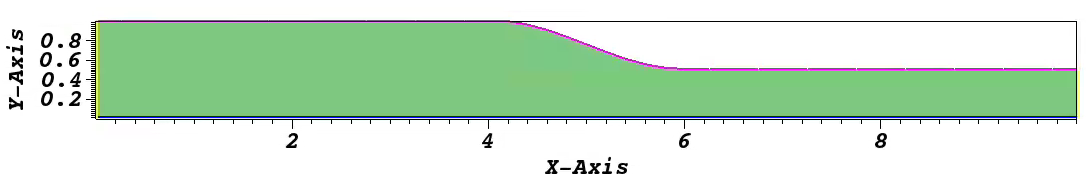
\includegraphics[width=0.7\linewidth]{geom.png}
		\caption{Géometrie de GDL (2D)}
		\label{fig:geom}
	\end{figure}
	
	\justify
	La dimension est la suivante:
	\begin{itemize}
		\item largeur (horizontale, Ox) 10
		\item épaisseur (vertical, Oy):
			\begin{itemize}
				\item zone non écrasé: épaisseur à 1
				\item zone écrasé: épaisseur à 0.5
			\end{itemize} 
	\end{itemize}
	
	Quatre bords sont définie: Gauche et Droit (jaune), Haut (violet) et Bas (bleue)
	
	\paragraph{Modèle mathématique}
	On considère la Conduction de la Chaleur dont l'équation comprend une opérateur de diffusion avec le coefficient anisotrope matriciel:
	\begin{equation}
		div(-Dgrad(T)) = q
	\end{equation}
		
	avec:\\
	T température $K$ \\
	q source par e.x. densité du flux de chaleur $W/m^2$ \\
	D coefficient de conductivité, $W/m/K$. Dans le cas d'anisotropie, il s'agit d'une matrice de taille 3x3 en tridimensionnel et 2x2 en bidimensionnel. La forme de matrice D dépend de la zone sur la géométrie:\\
	
	\begin{itemize}
		\item zone sur laquelle le bord est droit, non incliné: D est diagnonale \\
		$ D = \left( 
			\begin{matrix}
			D_{xx} & 0 & 0\\
			0 & D_{yy} & 0\\
			0 & 0 & D_{zz}\\
			\end{matrix} 
			\right) $
		avec $ D_{xx} = D_{zz} >> D_{yy} $
		\item zone dont le bord est courbé et incliné: D est pleine symétrique \\
		$ D = \left( 
		\begin{matrix}
		D_{xx} & D_{xy} & D_{xz}\\
		- & Dyy & D_{yz}\\
		- & - & D_{zz}\\
		\end{matrix} 
		\right) $ 
		avec $ D_{diagonal} >> D_{extra-diagnonal} $ \\
		La matrix D dans cette zone est le produit matriciel $D = M.D_{diagonal}.M^{-1}$ avec M la matrice de rotation (unitaire) en fonction de l'angle d'inclination.
		\begin{itemize}
			\item en 2D: \\ 
			$ M = \left( 
			\begin{matrix}
			\cos(\theta) & \sin(\theta)\\
			-\sin(\theta) & \cos(\theta)\\
			\end{matrix} 
			\right) $
			\item en 3D \\
			$ M = \left[ 
			\begin{matrix}
			M_{xx} & M_{xy} & M_{xz}\\
			M_{yx} & M_{yy} & M_{yz}\\
			M_{zx} & M_{zy} & M_{zz}\\
			\end{matrix} 
			\right]  
			= \left[ \vec{u}, \vec{v}, \vec{w} \right] $ \\
			avec $\vec{v} = \nabla T(\theta)$ vecteur normal du plan de bord d'écrasement GDL, \\ 
			$\vec{u} = \vec{v} \times \vec{OY}$, \\ 
			$\vec{w} = \vec{v} \times \vec{u}$ \\
			La propriétaire de la matrice est $ M^{-1} = M^T$ et $\det{M}=1$ \\
		\end{itemize} 
		
		\item zone d'écrasement: la magnitude de D dépend linéairement aux valeurs de conductivité de la zone non écrasement et écrasement qui correspondent respectivement à l'épaisseur maximal et minimal de GDL. \\
		$ \alpha = \frac{ep-ep_{ec}}{ep_{non\_ec}-ep_{ec}} $ \\
		
		$ D = \alpha D_{non\_ec}+(1-\alpha) D_{ec} $ \\
	\end{itemize}
	
	\paragraph{Condition limite}
	\begin{itemize}
		\item adiabatique sur les bords Gauche et Haut \\
		\item dirichlet $ T = 0 $ sur le bord Bas \\
		\item température externe imposé $ T = 1 $ avec coefficient d'échange imposé mix \\
		\begin{itemize}
			\item zone non écrasement ($ x = [0, 4] $) h\_imp égale à 0. \\
			\item zone écrasement ($x = [6, 10]$) h\_imp égale à 10. \\
			\item zone transitoire ($x = (4, 6)$) h\_imp est en fonction de x (continue)
			 $ 10.0,5(1.+ \sin(0,5\Pi(x-5))) $ \\
		\end{itemize}
	\end{itemize} \par

	\paragraph{Maillage}
	La discrétisation schéma utilise un non structuré maillage (VEF) \par
	
	\paragraph{Sonde}
	on crée deux sondes
	\begin{itemize}
		\item  le champ température sur la ligne diagonale de la géométrie P1(0,1) et P2(10,0)
		\item et le flux sur le bord Haut
	\end{itemize}
	
	\subsection*{MEDCoupling script}
	\textbf{Fichier MEDCoupling\_matrix\_aniso.py}
	\lstinputlisting[language=python]{MEDCoupling_matrix_aniso.py}
	
	\subsection*{Data fichier}

	\textbf{Fichier PEMFC\_2D\_aniso\_withMEDCouplingFull.data}
		\lstinputlisting[language=python]{PEMFC_2D_aniso_withMEDCouplingFull.data}
\end{document}
